\documentclass{article}
\usepackage[utf8]{inputenc}
\usepackage[T1]{fontenc}
\usepackage{amsmath}
\usepackage{amssymb}
\usepackage{hyperref}
\usepackage{listings}
\usepackage{xcolor}
\usepackage{tikz}
\usepackage{geometry}
\usepackage{float}
\usepackage{enumitem}
\usepackage{booktabs}

\geometry{a4paper, margin=1in}

\usetikzlibrary{shapes.geometric, arrows, positioning, calc, decorations.pathreplacing}

\definecolor{codegray}{rgb}{0.5,0.5,0.5}
\definecolor{codepurple}{rgb}{0.58,0,0.82}
\definecolor{backcolour}{rgb}{0.95,0.95,0.92}

\lstdefinelanguage{JavaScript}{
  keywords={break, case, catch, continue, debugger, default, delete, do, else, false, finally, for, function, if, in, instanceof, new, null, return, switch, this, throw, true, try, typeof, var, void, while, with},
  morekeywords={class, export, boolean, throw, implements, import, this},
  sensitive=true,
  morecomment=[l]{//},
  morecomment=[s]{/*}{*/},
  morestring=[b]',
  morestring=[b]"
}

\lstset{
    backgroundcolor=\color{backcolour},
    commentstyle=\color{green!60!black},
    keywordstyle=\color{magenta},
    numberstyle=\tiny\color{codegray},
    stringstyle=\color{codepurple},
    basicstyle=\ttfamily\footnotesize,
    breakatwhitespace=false,
    breaklines=true,
    captionpos=b,
    keepspaces=true,
    numbers=left,
    numbersep=5pt,
    showspaces=false,
    showstringspaces=false,
    showtabs=false,
    tabsize=2
}

\title{Timeline Layout Algorithm: Complete Technical Specification}
\author{Antigravity Implementation Team}
\date{January 2026}

\begin{document}

\maketitle

\begin{quote}
    \textbf{Core Concept}: ``Tetris with Rubber Bands'' \\
    A constrained force-directed layout algorithm that arranges team nodes on horizontal ``swimlanes'' while minimizing visual crossings and maintaining family proximity.
\end{quote}

\tableofcontents
\newpage

\section{Fundamental Definitions}

\subsection{What is a Node?}
A \textbf{Node} represents a single cycling team with properties defining its lifecycle and identity:

\begin{lstlisting}[language=JavaScript]
{
  id: "LPR",                    // Unique identifier
  founding_year: 2004,          // Year the team was founded
  dissolution_year: 2009,       // Year the team dissolved (or null if still active)
  eras: [                       // Array of yearly "slices"
    { year: 2004, name: "LPR Brakes" },
    { year: 2005, name: "LPR Brakes" },
    // ... one entry per year
  ]
}
\end{lstlisting}

\textbf{Visual Representation}: A node is drawn as a horizontal bar spanning from $founding\_year$ to $dissolution\_year + 1$ (inclusive rendering).

\textbf{Example}: LPR (2004--2009) visually occupies the space from year 2004 through the end of year 2009.

\subsection{What is Temporal Overlap?}
Two nodes \textbf{temporally overlap} if they exist at the same time. This is determined using \textbf{inclusive} year boundaries:

\begin{equation}
    Overlap(A, B) \iff (A_{start} \le B_{end}) \land (B_{start} \le A_{end})
\end{equation}

\textbf{Critical Edge Case - ``Touching'' Nodes}:
\begin{itemize}
    \item LPR ends 2009, Utensilnord starts 2010 $\implies$ \textbf{NO OVERLAP} ($2009 < 2010$)
    \item Sanson ends 1980, Famcucine starts 1980 $\implies$ \textbf{OVERLAP} ($1980 \le 1980$)
\end{itemize}

\textbf{Why this matters}: Nodes that overlap cannot share the same horizontal lane (swimlane) because they would visually collide.

\subsection{What is a Chain?}
A \textbf{Chain} is a linear sequence of nodes connected by 1-to-1 relationships with \textbf{no temporal overlap}.

\begin{lstlisting}[language=JavaScript]
{
  id: "chain-0",
  nodes: [LPR, Utensilnord, Katusha],  // Array of node objects
  startTime: 2004,                      // founding_year of first node
  endTime: 2019,                        // dissolution_year of last node
  yIndex: 0                             // Current lane assignment
}
\end{lstlisting}

\textbf{Chain Formation Rules}:
\begin{enumerate}
    \item \textbf{Linear Topology}: Each node has exactly 1 predecessor and 1 successor (except endpoints).
    \item \textbf{No Temporal Overlap}: Consecutive nodes must NOT overlap.
    \item \textbf{Break on Split/Merge}: If a node has multiple children or multiple parents, the chain breaks.
\end{enumerate}

\textbf{Example Chain}:
LPR (2004--2009) $\to$ Utensilnord (2010--2015) $\to$ Katusha (2016--2019) \\
These three nodes form ONE chain because they satisfy all rules and do not overlap ($2009 < 2010$ and $2015 < 2016$).

\textbf{Counter-Example (Chain Break)}:
Sanson (1963--1980) $\times$ Famcucine (1980--1981) \\
These form TWO separate chains because they overlap ($1980 \le 1980$).

\subsection{What is a Link?}
A \textbf{Link} represents a lineage connection between two teams:

\begin{lstlisting}[language=JavaScript]
{
  source: "LPR",           // Source node ID
  target: "Tinkoff",       // Target node ID
  type: "LEGAL_TRANSFER",  // Type of connection
  year: 2007               // Year the connection occurred
}
\end{lstlisting}

\textbf{Visual Representation}: Links are drawn as curved paths connecting the source node to the target node.

\subsection{What is a Vertical Segment?}
When a link connects nodes in different lanes, it creates a \textbf{Vertical Segment} - the portion of the link that crosses intermediate lanes.

\begin{figure}[H]
    \centering
    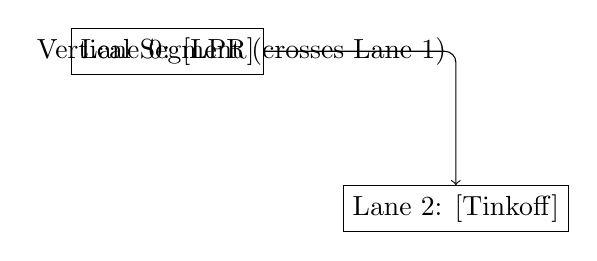
\begin{tikzpicture}
        \node (LPR) [draw, rectangle, minimum width=2cm] {Lane 0: [LPR]};
        \node (Tinkoff) [right=of LPR, yshift=-2cm, draw, rectangle, minimum width=2cm] {Lane 2: [Tinkoff]};
        \draw[->, rounded corners] (LPR.east) -| node[pos=0.5, left] {Vertical Segment (crosses Lane 1)} (Tinkoff.north);
    \end{tikzpicture}
\end{figure}

\textbf{Key Property}: A vertical segment exists at a specific \textbf{year} (the link's year) and spans between two \textbf{lanes}.

\subsection{What is a Cut-Through?}
A \textbf{Cut-Through} occurs when a node sits in a lane that a vertical segment passes through.

\begin{figure}[H]
    \centering
    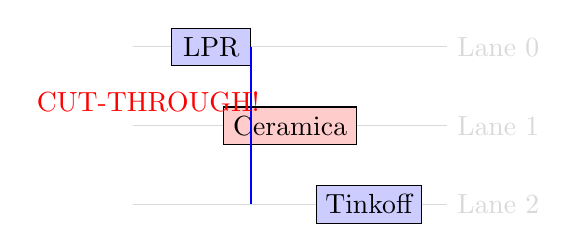
\begin{tikzpicture}
        \draw[gray!30] (0,1) -- (4,1) node[right] {Lane 0};
        \draw[gray!30] (0,0) -- (4,0) node[right] {Lane 1};
        \draw[gray!30] (0,-1) -- (4,-1) node[right] {Lane 2};
        
        \node at (1,1) [draw, fill=blue!20, minimum width=1cm] {LPR};
        \node at (2,0) [draw, fill=red!20, minimum width=1cm] {Ceramica};
        \node at (3,-1) [draw, fill=blue!20, minimum width=1cm] {Tinkoff};
        
        \draw[thick, blue] (1.5,1) -- (1.5, -1);
        \node[red] at (0.2, 0.3) {CUT-THROUGH!};
    \end{tikzpicture}
\end{figure}

\textbf{Detection Logic}:
\begin{lstlisting}[language=JavaScript]
// For a node in lane Y, check all vertical segments
isCutThrough = (
  Y > segment.y1 &&           // Node is between the two lanes
  Y < segment.y2 &&
  segment.time >= node.start && // Link occurs during node's lifetime
  segment.time <= node.end + 1  // +1 accounts for inclusive rendering
)
\end{lstlisting}

\textbf{Why +1?} Since nodes render inclusively to $dissolution\_year + 1$, a node ending in 2009 visually extends to the start of 2010. A link at year 2010 should detect a cut-through with this node.

\subsection{What is a Blocker?}
A \textbf{Blocker} occurs when a node sits on top of a vertical segment, blocking the visual ``corridor'' between parent and child.

\textbf{Key Difference from Cut-Through}:
\begin{itemize}
    \item \textbf{Cut-Through}: The link slices through the node (node is the victim).
    \item \textbf{Blocker}: The node blocks someone else's link (node is the perpetrator).
\end{itemize}

\subsection{What is Lane Sharing?}
\textbf{Lane Sharing} occurs when multiple chains occupy the same horizontal lane.

\textbf{Strict Stranger Rule}: Unrelated chains (``strangers'') are \textbf{strictly forbidden} from sharing a lane unless there is at least a 1-year gap between them. Since nodes render to $dissolution\_year + 1$:
\begin{itemize}
    \item Node A ends in 2009 (renders to 2010)
    \item Node B starts in 2011
    \item Gap = 2011 - 2010 = 1 year $\checkmark$ (allowed)
\end{itemize}

\textbf{Family Exception}: Parent and child chains can share lanes with temporal overlap.

\textbf{Distance Decay} (Currently Disabled): The penalty formula remains but with weight = 0:
\begin{equation}
    Penalty = \frac{W_{SHARE}}{\max(0.5, \Delta T)}
\end{equation}

\section{Math Symbols \& Variables Reference}
To clarify the formulas used in the optimization phases, here is a reference of the symbols and variables:

\begin{table}[H]
    \centering
    \begin{tabular}{lp{3cm}p{8cm}}
        \toprule
        \textbf{Symbol} & \textbf{Name} & \textbf{Description} \\
        \midrule
        $Y$ & \textbf{Lane Index} & The vertical coordinate of a chain (0 = top). \\
        $T$ & \textbf{Time} & An integer year (e.g., 2007). \\
        $\mu_{parents}$ & \textbf{Mean Parent Lane} & Average $Y$ position of all parent chains connected to current chain. \\
        $\mu_{children}$ & \textbf{Mean Child Lane} & Average $Y$ position of all child chains connected to current chain. \\
        $\Delta T$ & \textbf{Temporal Gap} & Years between two nodes. Positive = gap, negative = overlap. \\
        $J$ & \textbf{Total Cost} & The "energy" of a specific lane assignment to be minimized. \\
        $W_{XXX}$ & \textbf{Weights} & Penalty multipliers defining constraint importance. \\
        $P$ & \textbf{Parent Lane} & The $Y$ coordinate of an individual parent chain. \\
        $C$ & \textbf{Child Lane} & The $Y$ coordinate of an individual child chain. \\
        \bottomrule
    \end{tabular}
    \caption{Math Symbols and Variables}
\end{table}

\section{Algorithm Overview}

\begin{figure}[H]
    \centering
    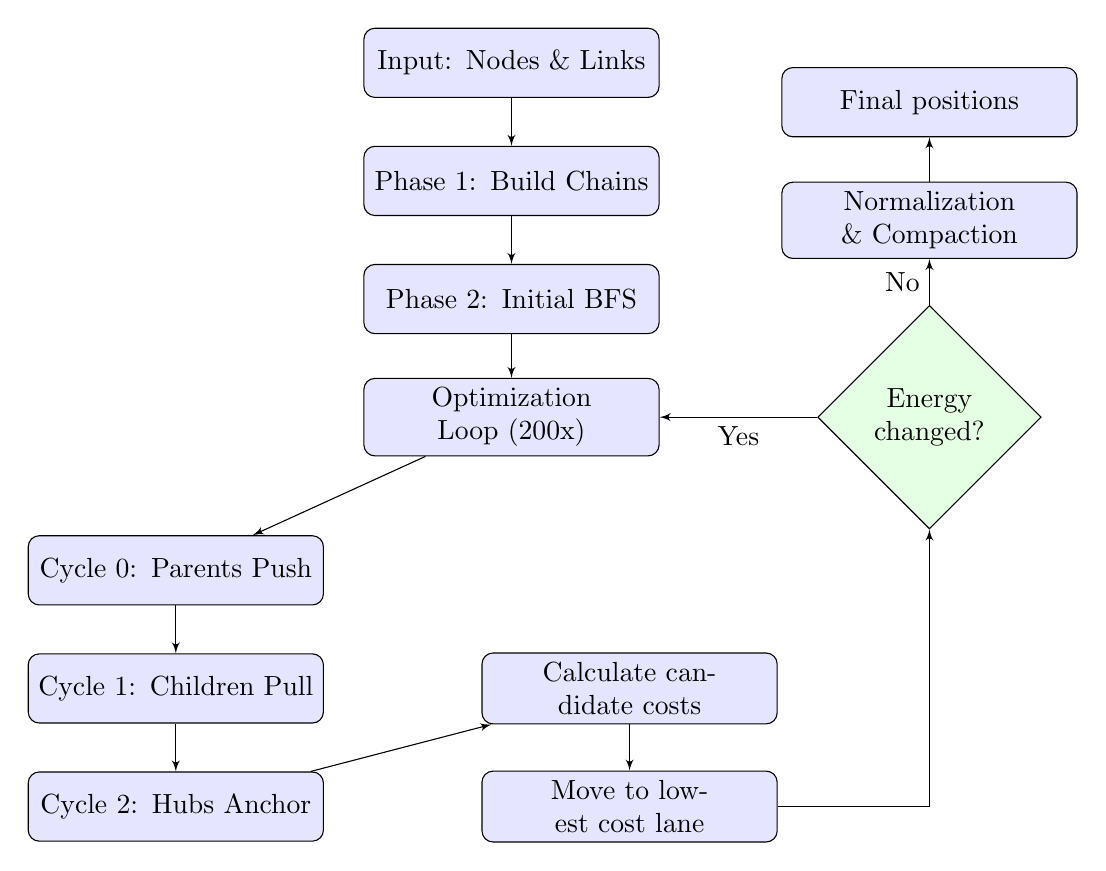
\begin{tikzpicture}[node distance=1.5cm, auto]
        \tikzstyle{block} = [rectangle, draw, fill=blue!10, text width=10em, text centered, rounded corners, minimum height=2.5em]
        \tikzstyle{decision} = [diamond, draw, fill=green!10, text width=6em, text centered, inner sep=0pt]
        \tikzstyle{line} = [draw, -latex']
        
        \node [block] (input) {Input: Nodes \& Links};
        \node [block, below of=input] (phase1) {Phase 1: Build Chains};
        \node [block, below of=phase1] (phase2) {Phase 2: Initial BFS};
        \node [block, below of=phase2] (opt) {Optimization Loop (200x)};
        
        \node [block, below left=1cm and 0.5cm of opt] (cycle0) {Cycle 0: Parents Push};
        \node [block, below of=cycle0] (cycle1) {Cycle 1: Children Pull};
        \node [block, below of=cycle1] (cycle2) {Cycle 2: Hubs Anchor};
        
        \node [block, right=2cm of cycle1] (cost) {Calculate candidate costs};
        \node [block, below of=cost] (move) {Move to lowest cost lane};
        \node [decision, right=2cm of opt] (energy) {Energy changed?};
        
        \node [block, above of=energy, node distance=2.5cm] (norm) {Normalization \& Compaction};
        \node [block, above of=norm] (output) {Final positions};

        \path [line] (input) -- (phase1);
        \path [line] (phase1) -- (phase2);
        \path [line] (phase2) -- (opt);
        
        \path [line] (opt) -- (cycle0);
        \path [line] (cycle0) -- (cycle1);
        \path [line] (cycle1) -- (cycle2);
        \path [line] (cycle2) -- (cost);
        \path [line] (cost) -- (move);
        \path [line] (move) -| (energy);
        \path [line] (energy) -- node {No} (norm);
        \path [line] (energy) -- node {Yes} (opt);
        \path [line] (norm) -- (output);
    \end{tikzpicture}
    \caption{Layout Algorithm Pipeline}
\end{figure}

\section{Phase 1: Chain Decomposition}
\textbf{Goal}: Group nodes into rigid linear units that move together.

\textbf{Algorithm}:
\begin{enumerate}
    \item Build predecessor/successor maps from links.
    \item For each unvisited node:
    \begin{enumerate}
        \item If it's a chain start (0 or $>1$ predecessors):
        \begin{itemize}
            \item Walk forward following single successors.
            \item Stop if: no successor, $>1$ successors, or temporal overlap.
            \item Create chain from collected nodes.
        \end{itemize}
        \item Mark all nodes in chain as visited.
    \end{enumerate}
\end{enumerate}

\section{Phase 2: Initial Placement}
\textbf{Goal}: Create a starting layout using Breadth-First Search (BFS).
Root chains are placed first (lane 0), then descendants are searched for the first available non-overlapping lane.

\section{Phase 3: Optimization Loop}

\subsection{Iteration Strategy (Tri-State Cycle)}
The loop alternates between three sorting strategies every iteration:
\begin{itemize}
    \item \textbf{Cycle 0 - Parents Push}: Sort by $startTime$ ASC.
    \item \textbf{Cycle 1 - Children Pull}: Sort by $startTime$ DESC.
    \item \textbf{Cycle 2 - Hubs Anchor}: Sort by $degree$ DESC.
\end{itemize}

\subsection{Candidate Search Strategy}
For each chain at current lane $Y$, the algorithm searches:
\begin{enumerate}
    \item \textbf{Local Neighborhood}: $Y \pm 50$ lanes.
    \item \textbf{Parent Vicinity}: $P \pm 10$ lanes.
    \item \textbf{Child Vicinity}: $C \pm 10$ lanes.
\end{enumerate}

\section{Cost Function Details}

The total cost $J$ for a chain considering lane $Y$ is:
\begin{equation}
    J = C_{ATTR} + C_{CUT} + C_{BLOCK} + C_{SHARE} + C_{YSHAPE}
\end{equation}

\subsection{Attraction Cost ($C_{ATTR}$)}
\textbf{Formula}: $C_{ATTR} = W_{ATTR} \times (|Y - \mu_{parents}|^2 + |Y - \mu_{children}|^2)$ \\
\textbf{Weight}: 100 \\
\textbf{Example}: Chain at $Y=5$ with parents at average lane 3 and children at average lane 8. \\
$C_{ATTR} = 100 \times ((5-3)^2 + (5-8)^2) = 100 \times (4 + 9) = 1,300$.

\subsection{Cut-Through Cost ($C_{CUT}$)}
\textbf{Formula}: $C_{CUT} = W_{CUT} \times (\text{Number of cuts})$ \\
\textbf{Weight}: 10,000 \\
\textbf{Example}: Chain Ceramica [2005--2010] at $Y=1$. Segment LPR(0) $\to$ Tinkoff(2) at 2007. \\
$Y=1$ is between 0 and 2; 2007 is within [2005, 2010] $\implies$ 1 cut. \\
$C_{CUT} = 10,000 \times 1 = 10,000$.

\subsection{Blocker Cost ($C_{BLOCK}$)}
\textbf{Formula}: $C_{BLOCK} = W_{BLOCK} \times (\text{Number of segments blocked})$ \\
\textbf{Weight}: 5,000

\subsection{Lane Sharing Cost ($C_{SHARE}$)}
\textbf{Formula}: $C_{SHARE} = W_{SHARE} / \max(0.5, \Delta T)$ \\
\textbf{Weight}: 0 (disabled)

\textbf{Strict Rule}: Strangers must have $\geq$ 1-year gap or lane is forbidden. Family can overlap.

\subsection{Y-Shape Symmetry Cost ($C_{YSHAPE}$)}
\textbf{Formula}: $C_{YSHAPE} = W_{YSHAPE} \times (\text{Number of violations})$ \\
\textbf{Weight}: 150

\section{Normalization \& Compaction}
\begin{enumerate}
    \item \textbf{Normalization}: $Y_{final} = Y - Y_{min}$.
    \item \textbf{Compaction}: Shift lanes to remove empty horizontal gaps.
\end{enumerate}

\section{Configuration Parameters}
\begin{lstlisting}[language=JavaScript]
export const LAYOUT_CONFIG = {
  ITERATIONS: { MIN: 50, MAX: 500, MULTIPLIER: 10 },
  SEARCH_RADIUS: 50,
  TARGET_RADIUS: 10,
  WEIGHTS: {
    ATTRACTION: 100.0,
    CUT_THROUGH: 10000.0,
    BLOCKER: 5000.0,
    LANE_SHARING: 0.0,      // Disabled (strict collision handles strangers)
    Y_SHAPE: 150.0
  }
};
\end{lstlisting}

\section{Known Limitations}
\begin{itemize}
    \item \textbf{Local Optimization}: Greedy nature can lead to jitter or local minima.
    \item \textbf{Asymmetric Penalties}: Mover pays the cost, potentially causing chains to "flee" each other.
    \item \textbf{Temporal Overlap Edge Cases}: Inclusive comparison ($>=$) prevents touch points.
\end{itemize}

\section{Debugging Tips}
\begin{itemize}
    \item \textbf{Visualizing Costs}: Log output of \texttt{calculateCost} for specific node IDs.
    \item \textbf{Tracing Moves}: Log source and target lanes during optimization iterations.
\end{itemize}

\section{Glossary}
\begin{itemize}[noitemsep]
    \item \textbf{Node}: A single team with founding/dissolution years.
    \item \textbf{Chain}: Linear sequence of nodes with no temporal overlap.
    \item \textbf{Lane}: Horizontal swimlane (Y-coordinate).
    \item \textbf{Link}: Connection between two nodes (parent$\to$child).
    \item \textbf{Vertical Segment}: Portion of a link crossing intermediate lanes.
    \item \textbf{Cut-Through}: Node sitting in a lane crossed by another family's link.
    \item \textbf{Blocker}: Node blocks another family's vertical link.
\end{itemize}

\end{document}
